\documentclass{article}

    \usepackage{fancyhdr}
    \usepackage{extramarks}
    \usepackage{amsmath}
    \usepackage{amsthm}
    \usepackage{amsfonts}
    \usepackage{tikz}
    \usepackage{amssymb}
    \usepackage{subcaption}
    \usepackage{blkarray}
    \usetikzlibrary{arrows, automata}
    \usepackage{forest}

    


    \usepackage{enumitem}

    \setlist[enumerate,1]{start=0} % only outer nesting level


    \usepackage{tabulary}

\usepackage[newcommands]{ragged2e}

    \usetikzlibrary{trees}

    \newcommand{\question}{\textbf{Question:}}
    \newcommand{\answer}{\textbf{Answer:}}

    


    \usetikzlibrary{decorations.markings}
    \tikzstyle{vertex}=[circle, draw, inner sep=0pt, minimum size=6pt]
    \newcommand{\vertex}{\node[vertex]}

    
    \usepackage{amsmath}
    \usepackage{algorithm}
    \usepackage[noend]{algpseudocode}
    \usepackage[utf8]{inputenc}
    \usepackage{enumerate}
    \usepackage{geometry}
    \usepackage{mathtools}
    \usepackage{parskip}
    \usepackage{xifthen, xparse}
    
    \algdef{SE}[SUBALG]{Indent}{EndIndent}{}{\algorithmicend\ }%
    \algtext*{Indent}
    \algtext*{EndIndent}
    
    
    
    \usetikzlibrary{automata,positioning}
    
    %
    % Basic Document Settings
    %
    
    \topmargin=-0.45in
    \evensidemargin=0in
    \oddsidemargin=0in
    \textwidth=6.5in
    \textheight=9.0in
    \headsep=0.25in
    
    \linespread{1.1}
    
    \pagestyle{fancy}
    \lhead{\hmwkAuthorName}
    \chead{\hmwkClass\ \hmwkTitle}
    \rhead{\firstxmark}
    \lfoot{\lastxmark}
    \cfoot{\thepage}
    
    \renewcommand\headrulewidth{0.4pt}
    \renewcommand\footrulewidth{0.4pt}
    
    \setlength\parindent{0pt}
    
    %
    % Create Problem Sections
    %
    
    \newcommand{\enterProblemHeader}[1]{
        \nobreak\extramarks{}{Problem \arabic{#1} continued on next page\ldots}\nobreak{}
        \nobreak\extramarks{Problem \arabic{#1} (continued)}{Problem \arabic{#1} continued on next page\ldots}\nobreak{}
    }
    
    \newcommand{\exitProblemHeader}[1]{
        \nobreak\extramarks{Problem \arabic{#1} (continued)}{Problem \arabic{#1} continued on next page\ldots}\nobreak{}
        \stepcounter{#1}
        \nobreak\extramarks{Problem \arabic{#1}}{}\nobreak{}
    }
    
    \newcommand\rowop[1]{\scriptstyle\smash{\xrightarrow[\vphantom{#1}]{\mkern-4mu#1\mkern-4mu}}}
    
    \DeclareDocumentCommand\converttorows%
    {>{\SplitList{,}}m}%
    {\ProcessList{#1}{\converttorow}}
    \NewDocumentCommand{\converttorow}{m}
    {\ifthenelse{\isempty{#1}}{}{\rowop{#1}}\\}
    
    \DeclareDocumentCommand \rowops{m}
    {\;
     \begin{matrix}
    \converttorows {#1}
     \end{matrix}
     \; }
    
    \setcounter{secnumdepth}{0}
    \newcounter{partCounter}
    \newcounter{homeworkProblemCounter}
    \setcounter{homeworkProblemCounter}{1}
    \nobreak\extramarks{Problem \arabic{homeworkProblemCounter}}{}\nobreak{}
    
    %
    % Homework Problem Environment
    %
    % This environment takes an optional argument. When given, it will adjust the
    % problem counter. This is useful for when the problems given for your
    % assignment aren't sequential. See the last 3 problems of this template for an
    % example.
    %
    \newenvironment{homeworkProblem}[1][-1]{
        \ifnum#1>0
            \setcounter{homeworkProblemCounter}{#1}
        \fi
        \section{Problem \arabic{homeworkProblemCounter}}
        \setcounter{partCounter}{1}
        \enterProblemHeader{homeworkProblemCounter}
    }{
        \exitProblemHeader{homeworkProblemCounter}
    }
    
    %
    % Homework Details
    %   - Title
    %   - Due date
    %   - Class
    %   - Section/Time
    %   - Instructor
    %   - Author
    %
    
    \newcommand{\hmwkTitle}{SOFTENG250 Assignment \#5}
    \newcommand{\hmwkClass}{D.S. and Algorithms}
    \newcommand{\hmwkAuthorName}{\textbf{Nisarag Bhatt}}
   
    
    %
    % Title Page
    %
    
    \title{
        \vspace{2in}
        \textmd{\textbf{\hmwkClass:\ \hmwkTitle}}\\
        \textmd{\textbf{ID Number: \idnumber}}\\
        \textmd{\textbf{UPI: \upi}}\\
        \vspace{3in}
    }
    
    \author{\hmwkAuthorName}
    \date{}
    
    \renewcommand{\part}[1]{\textbf{\large Part \Alph{partCounter}}\stepcounter{partCounter}\\}
    
    %
    % Various Helper Commands
    %
    
    % Useful for algorithms
    \newcommand{\alg}[1]{\textsc{\bfseries \footnotesize #1}}
    
    % For derivatives
    \newcommand{\deriv}[1]{\frac{\mathrm{d}}{\mathrm{d}x} (#1)}
    
    % For partial derivatives
    \newcommand{\pderiv}[2]{\frac{\partial}{\partial #1} (#2)}
    
    % Integral dx
    \newcommand{\dx}{\mathrm{d}x}
    
    % Alias for the Solution section header
    \newcommand{\solution}{\textbf{\large Solution}}
    
    % Probability commands: Expectation, Variance, Covariance, Bias
    \newcommand{\E}{\mathrm{E}}
    \newcommand{\Var}{\mathrm{Var}}
    \newcommand{\Cov}{\mathrm{Cov}}
    \newcommand{\Bias}{\mathrm{Bias}}
    
    \begin{document}
    
    
    \pagebreak
    
    \begin{homeworkProblem}

        \textbf{Question}: Run the $Dijkstra(G,s)$ algorithm on graph $G$ in Figure $1$ of Lecture Note $9$, starting at $v$. 

        \textbf{Answer}: 

        \begin{table}[h]
            \centering
            \begin{tabular}{|l|l|l|}
            \hline
            Iteration & F & $d$ values for $v \in F$ \\ \hline
            0         & $v$  & $d(v)=0$ \\ \hline
            1         & $v,x$  &$d(v)=0$, $d(x)=2$ \\ \hline
            2         & $v,x,z$ &$d(v)=0$, $d(x)=2$, $d(z)=3$ \\ \hline
            3         & $v,x,z,c$  &$d(v)=0$, $d(x)=2$, $d(z)=3$, $d(c)=6$ \\ \hline
            4         & $v,x,z,c,y$  &$d(v)=0$, $d(x)=2$, $d(z)=3$, $d(c)=6$, $d(y)=6$ \\ \hline
            5         & $v,x,z,c,y,q$  & $d(v)=0$, $d(x)=2$, $d(z)=3$, $d(c)=6$, $d(y)=6$, $d(q)=7$ \\ \hline
            6         & $v,x,z,c,y,q,u$ & $d(v)=0$, $d(x)=2$, $d(z)=3$, $d(c)=6$, $d(y)=6$, $d(q)=7$, $d(u)=12$\\ \hline
            7         & $v,x,z,c,y,q,u,w$ & $d(v)=0$, $d(x)=2$, $d(z)=3$, $d(c)=6$, $d(y)=6$, $d(q)=7$, $d(u)=12$, $d(w)=13$\\ \hline
            \end{tabular}
        \end{table}

        \begin{table}[h]
            \centering
            \begin{tabular}{|l|l|l|l|}
            \hline
            Iteration & F & $d$ values for $v \notin F$ \\ \hline
            0         & $v$  & $d(x)=2, d(c)=6, d(z)=3$ \\ \hline
            1         & $v,x$  &$d(c)=6$, $d(z)=3$ \\ \hline
            2         & $v,x,z$ &$d(c)=6$, $d(y)=6$\\ \hline
            3         & $v,x,z,c$  &$d(y)=6$, $d(u)=12$ \\ \hline
            4         & $v,x,z,c,y$  &$d(u)=12$, $d(q)=7$ \\ \hline
            5         & $v,x,z,c,y,q$  & $d(u)=12$ \\ \hline
            6         & $v,x,z,c,y,q,u$ & $d(w)=13$\\ \hline
            7         & $v,x,z,c,y,q,u,w$ & \\ \hline
            \end{tabular}
        \end{table}

        \textbf{Explanation for each Iteration}
        
        \begin{itemize}
            \item At iteration $0$: The source vertex $v$ is added to $F$ , the relaxation process provides the estimates for vertices $x, c, z$
            \item At iteration $1$: Vertex $x$ is added to $F$
            \item At iteration $2$: Vertex $z$ is added to $F$ and Vertex $y$ has its distance estimated from $z$.
            \item At iteration $3$: Vertex $c$ is added to $F$ and Vertex $u$ has its distance estimated from $c$.
            \item At iteration $4$: Vertex $y$ is added to $F$ and Vertex q has its distance estimated from $y$.
            \item At iteration $5$: Vertex $q$ is added to $F$.
            \item At iteration $6$: Vertex $u$ is added to $F$ and Vertex $w$ has its distance estimated from $u$.
            \item At iteration $7$: Vertex $w$ is added to $F$ and algorithm terminates as every other vertex is unreachable.
        \end{itemize}
        
    \end{homeworkProblem}

    \pagebreak

    \begin{homeworkProblem}
        \textbf{Question}: Let $T$ be a heap tree (representing an Array $H$) of height $n$

        (a) What is the number of internal nodes of $T$ with exactly one child?
        
        \answer

        At most one node has exactly one child. Each parent can have at most, two child
nodes. Consider a heap represented by an array $A$ . When you insert a new node into the heap, the node is added to the first free array slot. This means that each if a parent only has one node, every parent before it, must have two children.
        So either number of internal nodes with exactly one child is either $0$ or $1$.

        (b) Explain why every leaf of $T$ is at distance $n$ or $n-1$ from the root of $T$.

        \answer

        Similarly to the answer above, when vertices are inserted, into a heap represented by an array $A$ , 
        they are inserted at the first free array slot. These new child nodes will not have any children, and therefore they are leafs. These leafs are at the furthest distance from the root, ie. the height of the heap, $n$. 
        Similarly, the parents of these leaves can potentially have no children, so they are also leaves, but at a distance of $n-1$.

    \end{homeworkProblem}

    \begin{homeworkProblem}
        \textbf{Question}: Let $G$ be a graph. A $k$-colouring of $G$ is a colouring of vertices with at most $k$ colours such that no two adjacent vertices have the same colour.
        
        (a) Describe $1$-colourable graphs.

        \answer 

        $1$-colourable graphs are graphs which have no edges, if the graph has no edges then you can colour each graph the same colour but as soon as you have an edge you need to apply different colours to the end vertices of that edge.
        
        (b) What is the minimal number of colors needed to colour a tree with more than 1 node. Explain your answer.

        \answer

        For a tree with more than one node, $2$ colours is enough. 

        This is because we can fix the color of the root node, then all its children can have a different color, then all of its children can have the first color and so forth so the minimal number of colours required is $2$.

        For example we can consider this tree (where root is coloured 1 then second layer is 2 then 1 and so forth): 

        \begin{figure}[H]
            \centering
            \begin{subfigure}[b]{0.3\textwidth}
                \centering
                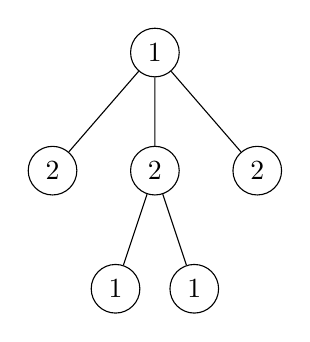
\begin{tikzpicture}[level distance=1.5cm,
                    level 1/.style={sibling distance=1.3cm},
                    level 2/.style={sibling distance=1cm}]
                    level 3/.style={sibling distance=0.8cm}]
                    \tikzstyle{every node}=[circle,draw]
                    \node (Root) {1}
                    child  {
                        node {2}
                    }
                    child  {
                        node {2} 
                        child { node {1} }
                        child { node {1} }
                    }
                    child {
                        node {2} 
                    };
                \end{tikzpicture}
                \centering
            \end{subfigure}
            \centering
        \end{figure}

        (c) Explain that the bipartite graph $K_{n,m}$ can be $2$-colourable.

        \answer 

        For $K_{n,m}$ we have that it can be $2$-colourable, why?

        Because we can assign $1$ to each vertex in the $n$ independent set and $2$ to each vertex in the $m$ independent set.

        For example consider the graph $K_{2,3}$ we can color all the $m$ vertices in red and all the $n$ vertices in blue so there are at most $2$ colours.

        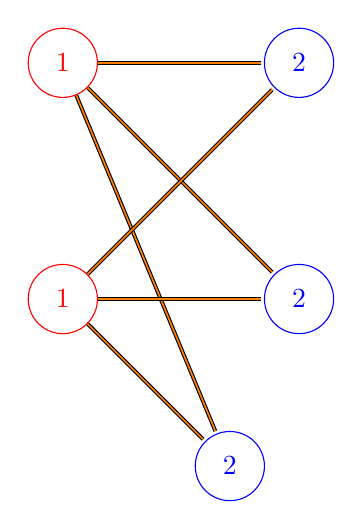
\begin{tikzpicture}[>=stealth',shorten >=1pt,node distance=3cm,on grid,initial/.style    ={}]
            \node[state] [red]         (a)                        {$1$};
            \node[state] [red]         (b) [below =of a]    {$1$};
            \node[state] [blue]        (c) [right =of a]    {$2$};
            \node[state]  [blue]           (d) [right =of b]    {$2$};
            \node[state]  [blue]           (e) [below right =of b]    {$2$};
            \tikzset{mystyle/.style={-,double=orange}} 
            \path (a)     edge [mystyle]    node  {} (c);
            \path (a)     edge [mystyle]    node  {} (d);
            \path (a)     edge [mystyle]    node  {} (e);
            \path (b)     edge [mystyle]    node  {} (c);
            \path (b)     edge [mystyle]    node  {} (d);
            \path (b)     edge [mystyle]    node  {} (e);
        \end{tikzpicture}

        

    \end{homeworkProblem}

    \begin{homeworkProblem}
        \question

        Let $k$ be the maximal among the degrees of all vertices of graph $G$. Write down a greedy
and linear / polynomial time algorithm that colours $G$ with at most $k + 1$ colours.

        \answer 

        Inputs: $G$ the graph

        Outputs: Coloured version of $G = G'$

        We can do the following steps for a greedy algorithm:
        
        \begin{itemize}
            \item Colour in the first vertex with the first colour
            \item For $k = 2$ to $|V|$ 
                \begin{itemize}
                    \item For the current vertex $V_k$ , colour it in with lowest numbered colour that has not been previously used on any \textbf{previously coloured vertices adjacent to it}.
                    \item If all previously used colours appear on vertices adjacent to $V_k$ then assign a new colour to $V_k$. 
                \end{itemize}
        \end{itemize}

        This algorithm is polynomial since you need to loop through all vertices and check adjacent vertices however with the help of adjacency matrices it is possible to make this algorithm linear. 
        
        This algorithm also colours $G$ with at most $k+1$ colours.



    \end{homeworkProblem}

    \pagebreak

    \begin{homeworkProblem}
        \question  
        
        Suppose $S = \{a,b,c,d,e,f\}$.  Give two examples of prefix codes for these letters. Present the
        prefix codes as binary trees.

        \answer

        Note that $|S|=6$ so there will be $6$ prefix codes.

        \begin{center}
            \includegraphics[scale = 0.2]{prefixtree.jpg}
        \end{center}  
                
    \end{homeworkProblem}



    \end{document}
    